\section{SONUÇ VE DEĞERLENDİRME}

\subsection{Sistem Performansı}

SmartWalk sistemi, ESP32-S3 kamera modülünün WiFi üzerinden sağladığı MJPEG akışını gerçek zamanlı olarak işleyerek yaya geçidi ihlallerini başarıyla tespit edebilmektedir. VGA (640$\times$480) çözünürlüğünde, her iki karede bir işleme (\texttt{FRAME\_SKIP=2}) yapılarak Python ortamında saniyede yaklaşık 10--15 kare işleme hızına ulaşılmıştır. YOLOv8n modelinin kişi ve araç tespitinde yeterli doğruluk sağladığı gözlemlenmiştir; kontrollü aydınlatma koşullarında güven eşiği \%40 olarak belirlenmiştir.

\subsection{İhlal Kaydı ve Bildirim}

İhlal anında kaydedilen fotoğraflar \texttt{violations/} klasörüne tarih damgalı dosya adlarıyla başarıyla kaydedilmiştir. Telegram üzerinden gönderilen bildirimler, fotoğraf eki ve tespit detaylarını (bölge içindeki araç ve yaya sayısı) içermektedir. 30 saniyelik cooldown mekanizması, ardışık karelerden kaynaklanan bildirim spamlenmesini etkin biçimde önlemiştir. Şekil~\ref{fig:ihlal}'de örnek bir ihlal görüntüsü, Şekil~\ref{fig:telegram}'de ise Telegram bildirim arayüzü sunulmaktadır.

\begin{figure}[H]
\centering
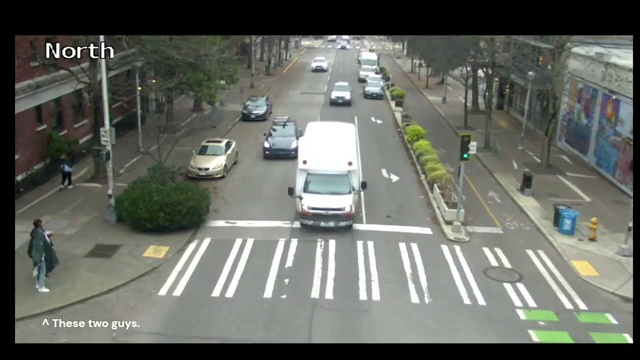
\includegraphics[width=0.65\textwidth]{ihlal_ornek.jpg}
\caption{Örnek ihlal anı fotoğrafı -- bölge içi araç ve yaya tespiti}
\label{fig:ihlal}
\end{figure}

\begin{figure}[H]
\centering
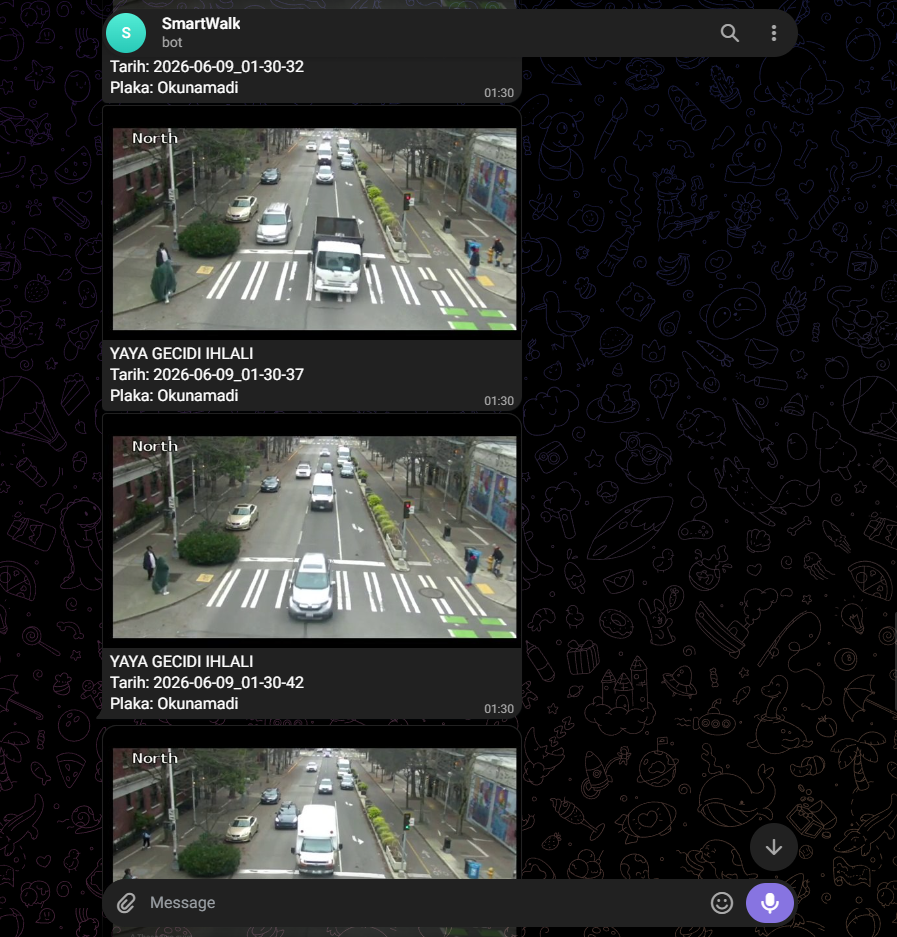
\includegraphics[width=0.42\textwidth]{telegram_ekran.jpg}
\caption{SmartWalk Telegram botu -- gerçek zamanlı ihlal bildirimleri}
\label{fig:telegram}
\end{figure}

\subsection{Sınırlamalar}

Sistemin mevcut sürümünde aşağıdaki sınırlamalar tespit edilmiştir:

\begin{itemize}
  \item \textbf{Disk alanı:} İhlal fotoğrafları silinmeden biriktiğinden, uzun süreli çalışmalarda disk alanı yönetimi manuel müdahale gerektirmektedir.
  \item \textbf{WiFi bağlantı kararlılığı:} ESP32 ile Python istemcisi arasındaki WiFi bağlantısının kesilmesi durumunda sistem otomatik yeniden bağlanma girişiminde bulunmakta, ancak kısa süreli kesintiler kare kaybına neden olmaktadır.
  \item \textbf{Aydınlatma koşulları:} Gece veya düşük aydınlatmalı ortamlarda YOLOv8n modelinin tespit doğruluğu düşmekte; bu durum ek ön işleme (CLAHE, parlaklık normalizasyonu) gerektirmektedir.
  \item \textbf{Yaya geçidi perspektif açısı:} Canny+Hough algoritması, kameraya dik olmayan yaya geçitlerinde (perspektif bozulması olan sahnelerde) başarısız olabilmekte; bu durumda manuel 4-nokta seçici devreye girmektedir.
\end{itemize}

\subsection{Gelecek Çalışmalar}

Projenin ilerleyen aşamalarında şu geliştirmeler planlanmaktadır:

\begin{itemize}
  \item \textbf{Plaka tanıma entegrasyonu:} \texttt{plate\_reader.py} modülünde altyapısı hazırlanmış olan EasyOCR tabanlı plaka okuma özelliğinin etkinleştirilmesi ve ihlal raporlarına plaka bilgisinin eklenmesi.
  \item \textbf{Gelişmiş model kullanımı:} Daha yüksek doğruluk gerektiren senaryolar için YOLOv8s veya YOLOv8m modellerine geçiş.
  \item \textbf{Bulut tabanlı izleme paneli:} Firebase verilerini görselleştiren bir web arayüzü geliştirilerek ihlal istatistiklerinin gerçek zamanlı takibinin sağlanması.
  \item \textbf{Çoklu kamera desteği:} Birden fazla ESP32 modülünün eş zamanlı yönetimi için dağıtık mimari tasarımı.
\end{itemize}

